\documentclass[a4paper,12pt,hidelinks]{report}

%%Pacchetti utili anche se non necessari

\usepackage{amsfonts}
\usepackage{amsmath}
\usepackage{latexsym}
\usepackage{tabularx}
\usepackage[italian]{babel}
\usepackage[bookmarks=true]{hyperref}
\usepackage{url}
% \usepackage{subfigure}
\usepackage{epstopdf}
\usepackage[utf8]{inputenc}
% \usepackage[utf8x]{inputenc}
\usepackage{listings}
\usepackage{graphicx}
%-------------------------------------------

% \title{Progettazione sito web\\ ''B\&B La Vecchia Posta''}
% \author{Daniele Di Pompeo \\mat. 226766}
% \annoaccademico{2013-2014}
\begin{document}
  \begin{titlepage}
    \begin{center}
    % Upper part of the page
      
\includegraphics[width=0.5\textwidth,keepaspectratio=true]{../img/logo}\\[1cm]    
      \textsc{\LARGE Piano di Qualità}\\[0.6cm]
      \textsc{\LARGE  progetto del sito:\\[0.5cm] ``B\&B La Vecchia Posta''}\\ [2.0cm]

    % Author and supervisor
      \begin{minipage}{0.8\textwidth}
	\begin{flushleft} \large
	  \emph{Autore:} Daniele Di Pompeo \\[0.5cm]
	  \emph{Versione documento: 1.1}\\[0.5cm]
	  \emph{Data emissione del documento: \today}\\[0.5cm]
	\end{flushleft}
      \end{minipage}
    \end{center}
  \end{titlepage}

\tableofcontents
 
\begin{abstract}
In questo documento viene descritto il piano di qualità relativo al documento dei requisiti del progetto del sito ``B\&B La Vecchia Posta''. Si analizzano gli aspetti 
critici del progetto, evidenziandone possibili soluzioni. Viene descritto il team di sviluppo, si fissano le milestone per la consegna del progetto.
\par Nella parte finale del progetto sono descritte le problematiche tecniche (configurazione dell'ambiente di sviluppo, configurazione server web, ecc.).
\end{abstract}

\chapter{Piano di qualità}
\section{Analisi dei rischi}
  \begin{center}
    \begin{tabular}{||m{4cm}|m{2.3cm}|m{2.3cm}|m{4cm}||}
      \hline
	\textbf{Descrizione del rischio} & \textbf{Probabilità che si verifichi} \textsuperscript{(1)} & \textbf{Gravità delle conseguenze} \textsuperscript{(2)} & \textbf{Azioni suggerite} \\
      \hline
	Guasti irreversibili sulla macchina utilizzata per lo sviluppo & bassa  & grave & utilizzo di versionamento su server remoti (utilizzato in particolare 
	il protocollo git del servizio gitHub)\\
      \hline
	Perdita del materiale multimediale per i contenuti & media & accettabile & backup del materiale su hard disk differenti e sincronizzazione 
	su server di versionamento\\
      \hline  
	Problemi con il servizio di hosting & media/alta & inaccetabile & individuare il servizio di hosting il più stabile possibile\\
      \hline
    \end{tabular}
    (1) alta / media / bassa \\
    (2) accettabile / grave / inaccetabile
  \end{center}

\section{Organizzazione del gruppo di progetto}
Per questo progetto il gruppo di sviluppo è costituito da una sola persona, il sottoscritto, che ricoprirà i ruoli di progettista, webmaster e capo-progetto.
\section{Responsabile del committente}
Non previsto per questo progetto essendo il committente e il progettista la stessa persona. 
\section{Piano di progetto}
Il piano di progetto viene mostrato sottoforma di Gantt Chart, con scala in giorni. Durante la fase di sviluppo verranno rilasciati diversi prototibi:
\begin{itemize}
 \item Prototipo di navigazione
 \item Prototipo di comunicazione
 \item Prototipo funzionale
 \item Prototipo editoriale
\end{itemize}
\begin{figure}[h!]%
    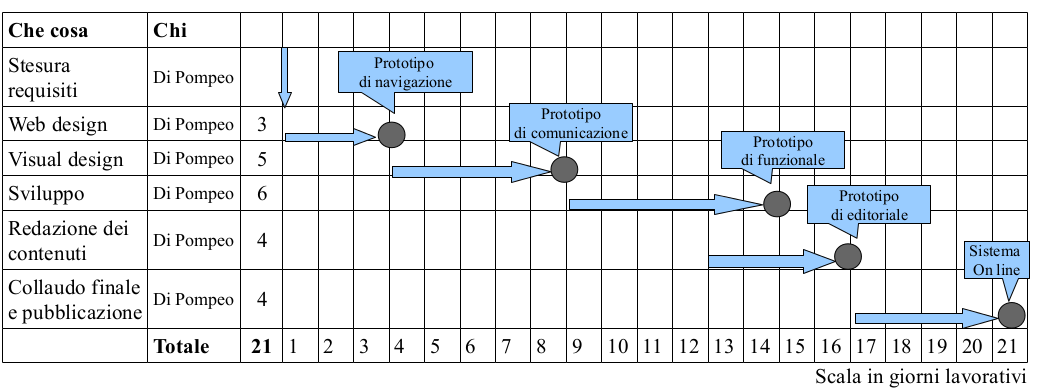
\includegraphics[width=1.2\textwidth,keepaspectratio=true]{../img/gantt_chart}
    \centering
    \caption{Gantt Chart del progetto}%
    \label{fig:gantt_chart}%
\end{figure}
Per la gantt chart si è scelto l'unità di misura in giorni lavorativi considerando che l'obiettivo della consegna è in 3 settimane di lavoro. 

\section{Controlli di avanzamento e rapporti}
Lo stato di avanzamento del progetto è legato alla volontà di consegnare il progetto entre le 3 settimane per ottenere sin da subito un feedback del lavoro svolto.

\section{Documentazione prevista}
I documenti redatti per lo sviluppo del progetto sono: 
\begin{enumerate}
 \item Documento dei requisiti
 \item Piano di qualità
 \item Prototipo di navigazione
 \item Prototipo di comunicazione
 \item Prototipo funzionale
 \item Prototipo editoriale
 \item Sito finale
\end{enumerate}
Tutta la documentazione sarà rilasciata gratuitamente tramite la repository di gitHub.

\section{Verifiche e convalide}
Dopo il rilascio di ogni prototipo, come indicato al punto 5, verranno eseguiti controlli e convalide sul lavoro svolto da parte del sottoscritto con l'aiuto di amici, estranei
al progetto. Si cercherà di eseguire test di usabilità almeno su due fasce di utenti, i più esperti di internet ed i meno esperti, per ottenere informazioni utili
sulle scelte prese.
\par Il collaudo finale sarà eseguito dal sottoscritto per verificarne la stabilità nei punti critici . Inoltre si conta di sottoporre il sito internet anche a persone
completamente inesperte di internet per testare la facilità di navigazione del sito.

\section{Consegna finale e pubblicazione del sito}
Convalidato tutti i prototipi si provvederà alla pubblicazione del sito web, sull'hosting scelto. Ioltre tutta la documentazione sarà consultabile attraverso la repository
github del progetto.

\section{Ambiente di sviluppo}
Il progetto sarà sviluppato nel seguente ambiente:
\begin{itemize}
 \item \textbf{Macchine}:
  \begin{itemize}
    \item Laptop Dell studio 1550 
    \item Laptop Asus k55
  \end{itemize}
 \item \textbf{Sistema operativo macchine di sviluppo}: Ubuntu 13.04 64bit, su entrambe le macchine
 \item \textbf{Server web locale}: XAMPP
 \item \textbf{CASE Tool}: Sparx Enterprise Architect
 \item \textbf{Framework di sviluppo}: beContent, framework dell'Università dell'Aquila del quale il sottoscritto è uno sviluppatore.
 \item \textbf{ServerSide}: PHP, come linguaggio di scripting e MySQL come DBMS
 \item \textbf{ClientSide}: HTML+CSS per il markup e Javascript, con plugin di jQuery e jQueryUI, come linguaggio di programmazione
\end{itemize}

\section{Gestione della configurazione}
Il framework utilizzato non necessita di particolari configurazioni essendo provvisto di uno script per l'installazione. Deve essere presente sulla macchina server un 
DBMS e un'interprete PHP. Inoltre bisogna indicare al framework il database che si vuole utilizzare.
\par \'E stato utilizzato il servizio di versionamento github sia per la documentazione sia per la parte di sviluppo del sito web.

\end{document}          
